\documentclass[12pt]{article}

\usepackage[utf8]{inputenc}
\usepackage{graphicx}

\title{Analyse de la fonction $\pi$\\Compte rendu}

\date{\today}

\begin{document}
\maketitle

\begin{abstract}
  Étude de la fonction $\pi$ de comptage du nombre de nombres
  premiers.
\end{abstract}

\section{Comparaison des fonctions $\pi(x)$ et $x/log(x)$}



\begin{figure}[h]
\caption{Courbes des fonctions $\pi(x)$ et $x/log(x)$}
\centering
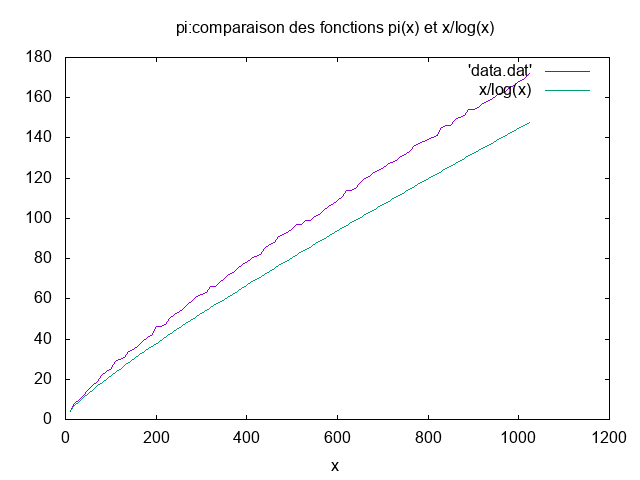
\includegraphics[width=0.5\textwidth]{pi}
\end{figure}

\section{Étude du temps de calcul}

\begin{figure}[h]
\caption{Temps de calcul de la fonction $\pi$}
\centering
\includegraphics[width=0.5\textwidth]{timing}
\end{figure}


\section{Étude de l'influence des options d'optimisation sur le temps
  de calcul}

\begin{figure}[h]
  \caption{Temps de calcul de la fonction $\pi(x)$ en fonction des
    options $-O1, -O2, -O3$}
\centering
\includegraphics[width=0.5\textwidth]{timingOx}
\end{figure}


\end{document}
